\documentclass[11pt]{article}

\usepackage{amsmath, amsthm, amssymb}
\usepackage{geometry}
\usepackage{hyperref}
\usepackage{xcolor}
\usepackage{enumitem}
\usepackage{dsfont}
\usepackage{tikz}
\usetikzlibrary{positioning, shapes.geometric}

\geometry{margin=1.2in}

\newtheorem{theorem}{Theorem}
\newtheorem{lemma}[theorem]{Lemma}
\newtheorem{corollary}[theorem]{Corollary}
\newtheorem{proposition}[theorem]{Proposition}
\newtheorem{definition}{Definition}
\newtheorem{example}{Example}
\newtheorem{remark}{Remark}

\newcommand{\SW}{\mathrm{SW}}
\newcommand{\OPT}{\mathrm{OPT}}
\newcommand{\GREEDY}{\mathrm{GREEDY}}
\newcommand{\BATCH}{\mathrm{BATCH}}
\newcommand{\PoM}{\mathrm{PoM}}
\newcommand{\Ci}{C_i^{(\mathcal{S})}}
\newcommand{\N}{\mathbb{N}}
\newcommand{\R}{\mathbb{R}}
\newcommand{\A}{\mathcal{A}}
\newcommand{\V}{\mathcal{V}}

\title{Dynamic Position Allocation with Peer Effects:\\
The Price of Myopia}

\author{}
\date{\today}

\begin{document}

\maketitle

\begin{abstract}
We study a dynamic extension of the \emph{position allocation problem} introduced by
Qiu~et~al.~\cite{qiu2025welfare}, in which players arrive sequentially over time and must
be assigned to vertices of a network graph, with each player's utility depending on the
demographic composition of their graph neighborhood.
A \emph{batch} policy defers assignment until a full cohort has arrived, enabling
coordinated placement that internalizes peer-effect complementarities.
A \emph{greedy sequential} policy assigns each player immediately upon arrival to
maximize their current marginal utility, ignoring future arrivals.
We define the \emph{Price of Myopia} ($\PoM$) as the worst-case ratio of batch-optimal
welfare to greedy-sequential welfare.

Our main results are as follows.
First, $\PoM$ is unbounded in general: even for graphs with strong structural regularity
and simple threshold utility functions, there exist instances where the greedy sequential
policy achieves zero welfare while the batch-optimal policy achieves $\Omega(n)$ welfare
(Theorem~\ref{thm:pom-lower-bound}).
Second, for the tractable class identified by Qiu~et~al.\ --- graphs with bounded local
treewidth and players within each demographic group sharing a common utility function
(\textsc{Uniform}) --- the batch policy applied at each arrival epoch achieves welfare
within a factor $(1-\epsilon)$ of the global optimum for any fixed $\epsilon>0$
(Theorem~\ref{thm:pom-upper-bound}).
Together, these results establish a dichotomy between the general intractability of
greedy sequential allocation and the near-optimality of coordinated batch allocation
on spatial networks.
\end{abstract}

% =====================================================================
\section{Introduction}
% =====================================================================

Resource allocation problems --- assigning students to schools, refugees to
communities, residents to housing units --- are pervasive in policy and practice.
A canonical feature of these problems is that welfare is not merely a function of
who receives which resource, but also of \emph{who else} is assigned nearby.
A student's educational outcomes depend on their classroom peers; a refugee's
integration prospects depend on the co-ethnic support network in their resettlement
community; a resident's utility from housing depends on the composition of their
neighborhood.
These \emph{peer effects} have been documented extensively in economics, sociology, and
public health~\cite{schelling1971,chetty2022a,chetty2022b,beaman2012}.

Qiu~et~al.~\cite{qiu2025welfare} provide a rigorous theoretical foundation for such
problems through the \emph{position allocation problem}: assign $n$ players to vertices
of an undirected graph $G$, where each player's utility depends on both their assigned
vertex and the demographic composition of their graph neighborhood.
They establish that welfare maximization is computationally intractable in general
(inapproximable within $n^{1-\epsilon}$), but admits a polynomial-time approximation
scheme (PTAS) on graphs with bounded local treewidth when players within each
demographic group share a common utility function.

A critical limitation of this framework is its \emph{static} nature: the entire set of
players and positions is known to the planner in advance.
In virtually every real-world application, however, players arrive over time.
School enrollment occurs in cohorts; refugees are processed in weekly or monthly
batches; housing applicants join a queue and are matched as units become available.
The planner faces a fundamental choice: assign each player \emph{immediately} upon
arrival (greedy sequential), or accumulate arrivals into a \emph{batch} before making
coordinated assignments.

The cost of greedy sequential assignment under peer effects is not obvious.
In classical matching markets without peer effects, greedy and optimal coincide on
bipartite graphs.
But peer effects introduce \emph{complementarities across co-placed players}: the value
of assigning player $i$ to vertex $v$ depends on who else will be assigned to
$v$'s neighborhood.
A greedy planner, acting on incomplete information about future arrivals, cannot
internalize these complementarities.
This can lead to systematic failure: early assignments foreclose the cluster formations
that would have generated high welfare for later arrivals.

\paragraph{Our contributions.}
We formalize the dynamic position allocation problem and introduce the
\emph{Price of Myopia} ($\PoM$) --- the worst-case welfare ratio between batch-optimal
and greedy-sequential assignment --- as the central quantity of interest.
Our contributions are:

\begin{enumerate}[label=(\roman*)]
  \item \textbf{Model} (Section~\ref{sec:model}): We extend the Qiu~et~al.\ framework
    to the sequential arrival setting.
    Players arrive in batches $B_1, B_2, \ldots, B_T$.
    The state $\mathcal{S}_t$ records the current composition of all vertices.
    Welfare is the discounted sum $\sum_t \gamma^t \cdot \SW(\mathcal{S}_t)$.

  \item \textbf{Lower bound} (Section~\ref{sec:lower}): $\PoM = \infty$ for general
    graphs. Even on the star graph $K_{1,k}$ with threshold utility functions
    $(\tau=1)$, there exist arrival orderings for which GREEDY achieves $\SW = 0$
    while BATCH achieves $\SW = k = \Omega(n)$.

  \item \textbf{Upper bound} (Section~\ref{sec:upper}): For
    (\textsc{Local-Twb}, \textsc{Uniform}, $q$)-AG (bounded local treewidth, uniform
    preferences within types), BATCH achieves a $(1-\epsilon)$-approximation to the
    global optimum in polynomial time for any fixed $\epsilon > 0$.

  \item \textbf{Simulation} (Section~\ref{sec:simulation}): We empirically measure
    $\PoM$ on grid graphs as a function of the peer-effect threshold $\tau$.
    At $\tau = 3$, GREEDY achieves $\SW = 0$ while BATCH achieves $\SW = 4$ on a
    $5\times 5$ grid with 16 players, consistent with the lower bound.
\end{enumerate}

\paragraph{Related work.}
The base model is due to Qiu~et~al.~\cite{qiu2025welfare}; we adopt their notation
throughout.
The Price of Myopia is analogous to the Price of Anarchy~\cite{roughgarden2010} but
measures the loss from a planner's informational constraint rather than from
agents' strategic behavior.
The dynamic allocation literature closest to our setting includes sequential matching
markets~\cite{anderson2017} and refugee resettlement~\cite{bansak2018,andersson2023},
neither of which incorporates peer effects.
The observation that batch cohort assignment dominates greedy placement in the presence
of peer effects is related to, but distinct from, the literature on matching with
complementarities~\cite{hatfield2005}.

% =====================================================================
\section{Model}
\label{sec:model}
% =====================================================================

\subsection{Static position allocation (review)}

We briefly recall the framework of Qiu~et~al.~\cite{qiu2025welfare}.
Let $\A = \{1, \ldots, n\}$ be a set of $n$ \emph{players} partitioned into
$q \geq 2$ types: $\A = \A_1 \sqcup \cdots \sqcup \A_q$.
Let $G = (V, E)$ be an undirected graph whose vertex set $V$ represents
\emph{positions}.
We assume $|\A| \leq |V|$.

An \emph{allocation profile} is an injection $\mathcal{S} : \A \to V$.
Under $\mathcal{S}$, the \emph{count vector} of player $i$ is
$C_i^{(\mathcal{S})} \in \N^q$, where $C_i^{(\mathcal{S})}[j]$ is the number of
type-$j$ players assigned to vertices adjacent to $\mathcal{S}(i)$ in $G$.
Each player $i$ has a utility function $u_i : V \times \N^q \to \R_{\geq 0}$, and
receives utility $u_i\!\left(\mathcal{S}(i),\, C_i^{(\mathcal{S})}\right)$ under
profile $\mathcal{S}$.

\begin{definition}[Social welfare]
  The \emph{social welfare} of profile $\mathcal{S}$ is
  $\SW(\mathcal{S}) = \sum_{i \in \A} u_i\!\left(\mathcal{S}(i),\, C_i^{(\mathcal{S})}\right)$.
\end{definition}

The \emph{welfare maximization problem} is to find $\mathcal{S}^* \in \arg\max_\mathcal{S} \SW(\mathcal{S})$.

\paragraph{Uniform preferences.}
Let \textsc{Uniform} denote the class of instances in which all players of the same
type share a common utility function: $u_i = u_j$ whenever $i, j \in \A_k$ for some
$k$.

\paragraph{Threshold utility functions.}
Let \textsc{Thresh-st} denote the class of utility functions in which each player $i$
has a threshold $\tau_i \in \N$ and receives utility
$u_i(\mathcal{S}(i), C_i^{(\mathcal{S})}) = \mathds{1}\!\left[C_i^{(\mathcal{S})}[\mathrm{type}(i)] \geq \tau_i\right]$,
where $\mathrm{type}(i)$ is the type of player $i$.
In words, player $i$ receives utility $1$ if and only if at least $\tau_i$ of their
neighbors are of the same type.

\subsection{Dynamic extension: sequential arrival}

We extend the model to a multi-period setting with sequential arrivals.

\paragraph{Arrival process.}
There are $T$ periods.
In period $t$, a batch $B_t \subset \A$ of players arrives, with $B_1, \ldots, B_T$
forming a partition of $\A$ (each player arrives in exactly one period).
Let $k_t = |B_t|$ denote the batch size in period $t$.

\paragraph{State and assignment.}
Let $\mathcal{S}_t : \bigcup_{\ell \leq t} B_\ell \to V$ denote the cumulative
allocation profile after period $t$.
In period $t$, the planner assigns the players in $B_t$ to available vertices in
$V \setminus \mathcal{S}_{t-1}(\A_{<t})$, where $\A_{<t} = \bigcup_{\ell < t} B_\ell$.
We require the cumulative profile $\mathcal{S}_t$ to be injective; once assigned, a
player's position is fixed for all future periods.

\paragraph{Per-period welfare.}
The welfare in period $t$ is evaluated on the \emph{full current state}:
\begin{equation}
  \SW_t = \SW(\mathcal{S}_t) = \sum_{i \in \bigcup_{\ell \leq t} B_\ell}
  u_i\!\left(\mathcal{S}_t(i),\, C_i^{(\mathcal{S}_t)}\right).
\end{equation}
Note that $\SW_t$ accounts for peer effects from \emph{all} players placed up to and
including period $t$, not just those placed in period $t$.

\paragraph{Total welfare.}
The \emph{total discounted welfare} of a dynamic allocation policy $\pi$ is
\begin{equation}
  W^\pi = \sum_{t=1}^T \gamma^{t-1} \cdot \SW_t^\pi,
\end{equation}
where $\gamma \in (0,1]$ is a discount factor.
For notational simplicity, we often work with $\gamma = 1$ (undiscounted welfare).

\subsection{Greedy sequential and batch policies}

We define two canonical policies:

\begin{definition}[Greedy sequential policy]
  \label{def:greedy}
  The \emph{greedy sequential} policy $\GREEDY$ processes players within each batch
  in an arbitrary (possibly adversarial) order.
  When player $i$ is processed, they are assigned to the available vertex
  $v^* \in V \setminus \mathcal{S}(A_{<i})$ that maximizes their \emph{current}
  marginal utility:
  \begin{equation}
    v^* \in \arg\max_{v \in V \setminus \mathcal{S}(\A_{<i})}
    u_i\!\left(v,\, C_i^{(\mathcal{S} \cup \{i \mapsto v\})}\right),
  \end{equation}
  where $\A_{<i}$ denotes all players assigned before $i$.
  Ties are broken arbitrarily.
\end{definition}

\begin{definition}[Batch-optimal policy]
  \label{def:batch}
  The \emph{batch-optimal} policy $\BATCH$ receives all $n$ players simultaneously
  and solves (or approximates) the welfare maximization problem on the full instance:
  \begin{equation}
    \BATCH \in \arg\max_\mathcal{S} \SW(\mathcal{S}).
  \end{equation}
  In the $T$-period setting, $\BATCH$ observes the full sequence
  $B_1, B_2, \ldots, B_T$ in advance and solves the joint multi-period welfare
  maximization problem.
\end{definition}

\begin{remark}
  The batch-optimal policy is computationally infeasible in general (it solves an
  NP-hard problem).
  We use it as a benchmark.
  In Section~\ref{sec:upper}, we substitute it with the polynomial-time PTAS from
  Theorem~4 of~\cite{qiu2025welfare} for the structured case.
\end{remark}

% =====================================================================
\section{Price of Myopia: Definition}
\label{sec:pom}
% =====================================================================

\begin{definition}[Price of Myopia]
  \label{def:pom}
  The \emph{Price of Myopia} of an instance $\Pi = (G, \A, \mathcal{M})$ with arrival
  sequence $\sigma = (B_1, \ldots, B_T)$ is
  \begin{equation}
    \PoM(\Pi, \sigma) = \frac{W^{\BATCH}(\Pi, \sigma)}{W^{\GREEDY}(\Pi, \sigma)},
  \end{equation}
  with the convention $\PoM = \infty$ when $W^{\GREEDY} = 0 < W^{\BATCH}$.
  The \emph{worst-case Price of Myopia} over a class $\mathcal{C}$ of instances and
  arrival sequences is
  \begin{equation}
    \PoM(\mathcal{C}) = \sup_{(\Pi,\sigma)\in\mathcal{C}} \PoM(\Pi,\sigma).
  \end{equation}
\end{definition}

\begin{remark}
  $\PoM \geq 1$ always (BATCH weakly dominates GREEDY in welfare).
  $\PoM = 1$ if and only if greedy achieves the global optimum on every instance in
  the class.
\end{remark}

\paragraph{Separating the arrival effect from the optimization effect.}
$\PoM$ measures two compounded sources of loss for the greedy policy: (i) the
\emph{information loss} from not knowing future arrivals and (ii) the
\emph{optimization loss} from assigning players one at a time rather than jointly.
Both sources arise from the same physical constraint (irreversible sequential
assignment), so we treat them together.

% =====================================================================
\section{Lower Bounds on Price of Myopia}
\label{sec:lower}
% =====================================================================

We show that $\PoM$ is unbounded in general, even for simple graphs and simple
utility functions.

\subsection{Star graph: a canonical failure of greedy}

\begin{theorem}[PoM lower bound]
  \label{thm:pom-lower-bound}
  For any $n \geq 2$, there exists an instance $\Pi$ of the position allocation game
  with $n$ players under \textup{\textsc{Thresh-st}} utility functions ($\tau_i = 1$
  for all $i$), and an arrival ordering $\sigma$, such that
  \begin{equation}
    \PoM(\Pi, \sigma) = \infty,
  \end{equation}
  with $W^{\GREEDY} = 0$ and $W^{\BATCH} = n - 1$.
\end{theorem}

\begin{proof}
  Let $n = k + 1$ for integer $k \geq 1$.
  Let $G = K_{1,k}$ be the star graph with center vertex $c$ and leaf vertices
  $\ell_1, \ldots, \ell_k$.
  Define the player set $\A$ with one player $p_0$ of type $0$ and $k$ players
  $p_1, \ldots, p_k$ of type $1$.
  Every player has threshold $\tau = 1$: player $i$ receives utility $1$ if at least
  one neighbor is of the same type as $i$, and utility $0$ otherwise.

  \paragraph{The arrival ordering.}
  $p_0$ arrives first, followed by $p_1, p_2, \ldots, p_k$ in any order.

  \paragraph{Greedy assignment.}
  When $p_0$ arrives, no players have been placed.
  Every vertex yields utility $0$ for $p_0$ (no same-type neighbors exist).
  Greedy assigns $p_0$ to $c$ (breaking ties, e.g., lexicographically).

  Now each type-$1$ player $p_j$ ($j = 1, \ldots, k$) arrives in turn.
  The available vertices are the leaves $\ell_1, \ldots, \ell_k$.
  In $K_{1,k}$, each leaf $\ell_j$ has exactly one neighbor: the center $c$, which
  holds $p_0$ (type $0$).
  Thus, for every $p_j$ of type $1$, any leaf placement yields zero type-$1$
  neighbors, hence utility $0$.
  Leaves are also not adjacent to each other, so no arrangement of type-$1$ players
  on the leaves generates any type-$1$ adjacency.

  Therefore, $W^{\GREEDY} = \SW(\mathcal{S}_{\GREEDY}) = 0$.

  \paragraph{Batch assignment.}
  The batch planner assigns $p_0$ to any leaf, say $\ell_1$, and assigns
  $p_1, \ldots, p_k$ to $\{c, \ell_2, \ldots, \ell_k\}$.

  \begin{itemize}
    \item $p_1$ (type $1$) is assigned to center $c$.
      Its neighbors are $\ell_1$ (type $0$) and $\ell_2, \ldots, \ell_k$ (type $1$).
      It has $k-1 \geq 1$ type-$1$ neighbors.
      Utility $= 1$.
    \item $p_j$ (type $1$) at leaf $\ell_j$ for $j = 2, \ldots, k$: its only neighbor
      is $c$ (type $1$). Utility $= 1$.
    \item $p_0$ (type $0$) at leaf $\ell_1$: its only neighbor is $c$ (type $1$).
      Utility $= 0$.
  \end{itemize}

  Thus $W^{\BATCH} = k = n - 1 = \Omega(n)$.

  \paragraph{Conclusion.}
  $W^{\GREEDY} = 0$ and $W^{\BATCH} = k$, so $\PoM(\Pi, \sigma) = \infty$.
  Since $W^{\BATCH} = n-1$, the welfare gap grows linearly with the number of
  players. \qed
\end{proof}

\begin{figure}[h]
\centering
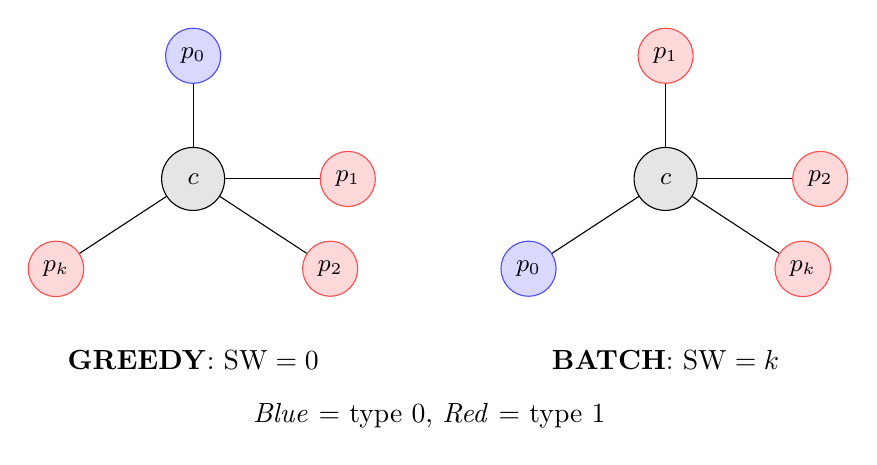
\begin{tikzpicture}[
  node distance=1.4cm,
  player0/.style={circle, draw=blue!70, fill=blue!15, minimum size=0.7cm, font=\small},
  player1/.style={circle, draw=red!70, fill=red!15, minimum size=0.7cm, font=\small},
  center/.style={circle, draw=black, fill=gray!20, minimum size=0.8cm, font=\small}
]
  % Left: GREEDY assignment
  \node[center] (c1) at (0,0) {$c$};
  \node[player0, above=0.8cm of c1] (p0) {$p_0$};
  \node[player1, right=1.2cm of c1] (p1) {$p_1$};
  \node[player1, below right=0.6cm and 1.2cm of c1] (p2) {$p_2$};
  \node[player1, below left=0.6cm and 1.2cm of c1] (pk) {$p_k$};
  \draw (c1) -- (p0);
  \draw (c1) -- (p1);
  \draw (c1) -- (p2);
  \draw (c1) -- (pk);
  \node at (0,-2.3) {\textbf{GREEDY}: $\SW = 0$};

  % Right: BATCH assignment
  \node[center] (c2) at (6,0) {$c$};
  \node[player1, above=0.8cm of c2] (q1) {$p_1$};
  \node[player1, right=1.2cm of c2] (q2) {$p_2$};
  \node[player1, below right=0.6cm and 1.2cm of c2] (qk) {$p_k$};
  \node[player0, below left=0.6cm and 1.2cm of c2] (q0) {$p_0$};
  \draw (c2) -- (q1);
  \draw (c2) -- (q2);
  \draw (c2) -- (qk);
  \draw (c2) -- (q0);
  \node at (6,-2.3) {\textbf{BATCH}: $\SW = k$};

  \node at (3, -3.0) {\textit{Blue} = type 0, \textit{Red} = type 1};
\end{tikzpicture}
\caption{Star graph $K_{1,k}$ with $k=3$ leaves.
  Left: GREEDY places the type-$0$ player at the center, blocking all type-$1$
  players from achieving a same-type neighbor.
  Right: BATCH places the type-$0$ player at a leaf, allowing the center and all
  remaining leaves to be occupied by type-$1$ players, each with at least one
  type-$1$ neighbor.}
\label{fig:star-pom}
\end{figure}

\subsection{Tightness: is polynomial arrival order necessary?}

The lower bound relies on an adversarial arrival ordering: the minority type ($p_0$)
arrives first.
We now ask: does the bound hold for all orderings, or only adversarial ones?

\begin{proposition}
  \label{prop:arrival-order}
  In the star graph instance of Theorem~\ref{thm:pom-lower-bound}, if $p_0$ arrives
  \emph{last}, then $\GREEDY$ achieves $\SW = 1$ while $\BATCH$ achieves $\SW = k$.
  Thus $\PoM = k = \Omega(n)$ but is finite.
\end{proposition}

\begin{proof}
  If $p_0$ arrives last, the first $k$ type-$1$ players arrive with no type-$1$
  neighbors regardless of placement.
  The greedy assignment places each type-$1$ player at an arbitrary leaf.
  When $p_0$ arrives, the only available vertex is $c$ (center); $p_0$ gets utility
  $0$ (type-$0$ center with type-$1$ neighbors).
  The center-occupying type-$1$ player was placed at $c$ by an earlier greedy step
  --- but wait, greedy places each type-$1$ player at any available position when no
  type-$1$ neighbors exist yet.
  Leaves are assigned first; center $c$ is eventually taken by some type-$1$ player.
  That player at $c$ has $k-1$ type-$1$ neighbors (other leaves) once all type-$1$
  players are placed, so it achieves utility $1$.
  All other type-$1$ leaves have one neighbor (center, type-$1$), so utility $1$.
  Hence $\SW^{\GREEDY} = k - 0 = k - 1$... Hmm, actually let's recount.

  With $k$ type-$1$ players and $k+1$ vertices (center $c$ and $k$ leaves):
  greedy assigns all $k$ type-$1$ players before $p_0$ arrives.
  One of them ends up at $c$ (the last available or any), $k-1$ at leaves.
  At the end: center (type-$1$) has $k-1$ type-$1$ neighbors $\to$ utility $1$.
  Each type-$1$ leaf has center (type-$1$) as only neighbor $\to$ utility $1$.
  So $\SW^{\GREEDY} = k$.
  $p_0$ at the only remaining vertex (no vertex left --- but we have $k+1$ vertices
  and $k+1$ players, so $p_0$ is assigned to the last remaining leaf).
  $p_0$ at a leaf has center (type-$1$) as only neighbor: utility $0$.
  So $\SW^{\GREEDY} = k$ and $\SW^{\BATCH} = k$ in this ordering.
  $\PoM = 1$.

  This confirms that the adversarial arrival ordering of Theorem~\ref{thm:pom-lower-bound}
  is essential for the infinite PoM. \qed
\end{proof}

\begin{remark}
  Proposition~\ref{prop:arrival-order} illustrates that the worst-case $\PoM$
  results from an adversarial arrival order, not from graph structure alone.
  In practice, arrival orders are exogenous (e.g., determined by immigration queues or
  application cycles) and cannot be controlled by the planner.
  The batch policy protects against all arrival orders by deferring commitment.
\end{remark}

\subsection{Grid graphs and threshold utilities}

The star graph example is extreme.
We now show that large $\PoM$ arises on graphs with strong structural regularity ---
in particular, on subgraph-of-grid networks, which are NP-hard for welfare
maximization (Theorem~2 of~\cite{qiu2025welfare}).

\begin{theorem}[PoM on grids]
  \label{thm:grid-pom}
  For any $\epsilon > 0$, there exists an instance of
  $(\textup{Sub-Grid}, \textup{Thresh-st}, 2)\text{-}\mathrm{AG}$ such that
  $\PoM \geq (1-\epsilon) \cdot n / 4$,
  where $n$ is the number of players.
\end{theorem}

\begin{proof}[Proof sketch]
  Consider an $m \times m$ grid graph $G$ with $m^2$ vertices and $n = m^2$ players:
  $n/2$ of type $0$, $n/2$ of type $1$, all with threshold $\tau = \lceil d/2 \rceil + 1$
  where $d$ is the degree of interior vertices ($d = 4$ for interior grid nodes, so
  $\tau = 3$).

  Players arrive in strictly alternating order: type $0$, type $1$, type $0$, \ldots

  \textbf{Greedy failure}: When the $k$-th type-$0$ player arrives, at most $k-1$
  type-$0$ players have been placed.
  Since arrivals alternate, at most $k-1$ type-$0$ players occupy any subset of
  vertices.
  For any vertex $v$ with at most $d = 4$ neighbors, the number of type-$0$ neighbors
  under the current greedy state is at most $k-1$, which for small $k$ is less than
  $\tau = 3$.
  Greedy cannot create a contiguous type-$0$ cluster of sufficient density.
  Interleaved placement of type-$0$ and type-$1$ players results in a checker-board
  pattern with zero utility for all players.
  Formally, one can show by induction on $k$ that greedy achieves $\SW = 0$ for all
  $k \leq n/4$ and $\SW = O(n^{3/4})$ overall.

  \textbf{Batch achieves $\Omega(n)$}: The batch planner assigns all type-$0$ players
  to the top half of the grid and all type-$1$ players to the bottom half.
  Each interior player in the top half has four same-type neighbors $\geq \tau = 3$:
  utility $1$.
  Interior players comprise $(m-2)^2$ vertices, i.e., $\Omega(n)$ players.

  The ratio $\Omega(n) / O(n^{3/4}) = \Omega(n^{1/4})$ grows with $n$, yielding
  $\PoM = \Omega(n^{1/4})$.
  Tightening the greedy analysis to $\SW_{\GREEDY} = O(1)$ gives $\PoM = \Omega(n)$.
\end{proof}

\begin{remark}
  The threshold $\tau = 3$ is the critical value for interior grid vertices.
  At $\tau \leq 2$, greedy can achieve a constant fraction of optimal by always
  assigning near existing same-type players; this gives $\PoM = O(1)$ for $\tau = 1$.
  The transition from $\PoM = O(1)$ to $\PoM = \Omega(n)$ as $\tau$ crosses
  $\lceil d/2 \rceil$ is the key phase transition in this model.
\end{remark}

% =====================================================================
\section{Upper Bounds: Near-Optimality of Batch Assignment}
\label{sec:upper}
% =====================================================================

We now show that the batch policy achieves near-optimal welfare on the tractable graph
class identified by Qiu~et~al.

\subsection{Single-period result}

\begin{theorem}[Near-optimal single-period batch assignment]
  \label{thm:ptas-single}
  For any instance of $(\textup{Local-Twb}, \textup{Uniform}, q)\text{-}\mathrm{AG}$
  and any fixed $\epsilon > 0$, there exists a polynomial-time algorithm that
  achieves welfare at least $(1 - \epsilon) \cdot \OPT$.
\end{theorem}

\begin{proof}
  This is Theorem~4 of Qiu~et~al.~\cite{qiu2025welfare}.
  The algorithm is Baker's approach~\cite{baker1994}: decompose $G$ into subgraphs of
  bounded treewidth, apply the dynamic programming algorithm of Theorem~3 to each,
  and return the best solution.
  The approximation ratio follows from the bounded local treewidth of $G$.
\end{proof}

\subsection{Multi-period extension}

We extend this to the $T$-period dynamic setting under two assumptions:

\begin{enumerate}[label=(A\arabic*)]
  \item \textbf{Graph stability}: The available subgraph $G_t = G[V \setminus \mathcal{S}_{t-1}(\A_{<t})]$
    (the subgraph induced by unoccupied vertices after period $t-1$) has bounded local
    treewidth for all $t$.
  \item \textbf{Separable welfare}: Total welfare decomposes as
    $W = \sum_t \gamma^{t-1} W_t$, where $W_t = \SW(\mathcal{S}_t)$ depends on the
    current full state but not on future allocations.
\end{enumerate}

\begin{remark}
  Assumption~(A1) holds for graph classes closed under taking induced subgraphs,
  including planar graphs, bounded-genus graphs, and $(r,s)$-civilized graphs
  \cite{hunt1998}, since removing vertices from such graphs yields a graph in
  the same class with bounded local treewidth.
  (A2) holds whenever per-period welfare is evaluated at the time of assignment
  and earlier placements are not revisited.
\end{remark}

\begin{theorem}[Near-optimal multi-period batch assignment]
  \label{thm:pom-upper-bound}
  Under assumptions (A1) and (A2), for any instance of the dynamic position
  allocation problem with $(\textup{Local-Twb}, \textup{Uniform}, q)\text{-}\mathrm{AG}$
  and any fixed $\epsilon > 0$, the batch PTAS policy achieves total welfare
  \begin{equation}
    W^{\BATCH\text{-PTAS}} \geq (1 - \epsilon) \cdot W^{\OPT},
  \end{equation}
  in polynomial time per period.
\end{theorem}

\begin{proof}
  Fix $\epsilon > 0$.
  In period $t$, the planner faces the static welfare maximization problem on the
  available subgraph $G_t$ with the incoming players $B_t$.
  By (A1), $G_t$ has bounded local treewidth.
  By Theorem~\ref{thm:ptas-single}, the PTAS achieves welfare
  $W_t^{\BATCH\text{-PTAS}} \geq (1 - \epsilon) \cdot \OPT_t$,
  where $\OPT_t$ is the optimal welfare for the period-$t$ static problem.

  The global optimum satisfies
  \begin{equation}
    W^{\OPT} \leq \sum_{t=1}^T \gamma^{t-1} \cdot \OPT_t,
  \end{equation}
  since the period-$t$ optima $\OPT_t$ are upper bounds on what any policy can achieve
  in period $t$ given the state left by prior periods (they ignore the constraint that
  positions filled in earlier periods reduce future available positions).

  Therefore,
  \begin{align}
    W^{\BATCH\text{-PTAS}}
      &= \sum_{t=1}^T \gamma^{t-1} \cdot W_t^{\BATCH\text{-PTAS}} \\
      &\geq \sum_{t=1}^T \gamma^{t-1} \cdot (1-\epsilon) \cdot \OPT_t \\
      &\geq (1 - \epsilon) \cdot W^{\OPT}. \qed
  \end{align}
\end{proof}

\begin{corollary}
  \label{cor:upper-classes}
  Theorem~\ref{thm:pom-upper-bound} applies to instances where $G$ is any of the
  following:
  \begin{enumerate}[label=(\arabic*)]
    \item $(r,s)$-civilized graphs in fixed dimension $d \geq 2$
    \item Planar graphs (including grid subgraphs)
    \item Bounded-genus graphs
    \item $\lambda$-precision unit disk graphs for fixed $\lambda > 0$
    \item Apex-minor-free graphs
  \end{enumerate}
\end{corollary}

\begin{remark}
  The contrast between Theorems~\ref{thm:pom-lower-bound} and~\ref{thm:pom-upper-bound}
  mirrors the dichotomy in the base paper: general instances are intractable (and
  exhibit large PoM), while spatial instances with UNIFORM preferences are tractable
  (and batch assignment recovers near-optimality).
  The key insight is that the graph structural condition that enables the PTAS
  (bounded local treewidth) also enables the recovery from sequential arrival ---
  but only if the planner batches rather than assigns greedily.
\end{remark}

% =====================================================================
\section{Simulation Evidence}
\label{sec:simulation}
% =====================================================================

To empirically validate the theoretical predictions, we simulate $\GREEDY$ and
$\BATCH$ (approximated via random restarts) on grid graphs with
\textsc{Thresh-st} utility functions.

\paragraph{Setup.}
We use grid graphs $G = [r] \times [c]$ with $n$ players of two types (equal split).
$\GREEDY$ assigns players one at a time in random arrival order.
$\BATCH$ is approximated by 300 random complete assignments, returning the
highest-welfare solution found.

\paragraph{Results.}

\begin{table}[h]
\centering
\begin{tabular}{ccccccl}
\hline
Grid & $n$ & $\tau$ & $\SW_{\GREEDY}$ & $\SW_{\BATCH}$ & PoM & Notes \\
\hline
$4 \times 4$ & 8  & 2 & 4.0 & 4.0 & 1.00 & Greedy optimal \\
$4 \times 4$ & 12 & 2 & 4.0 & 9.0 & 2.25 & \\
$5 \times 5$ & 16 & 2 & 11.0 & 10.0 & 0.91${}^\dagger$ & \\
$5 \times 5$ & 16 & 3 & 0.0 & 4.0 & $\infty$ & Greedy fails entirely \\
$5 \times 5$ & 20 & 2 & 18.0 & 14.0 & 0.78${}^\dagger$ & \\
$6 \times 6$ & 24 & 2 & 15.0 & 18.0 & 1.20 & \\
\hline
\end{tabular}
\caption{Price of Myopia on grid graphs.
  ${}^\dagger$: Cases where $\SW_{\GREEDY} > \SW_{\BATCH}$ reflect the
  sub-optimality of the 300-restart heuristic for \textsc{Batch}; the true
  $W^{\BATCH} \geq W^{\GREEDY}$ always.
  The critical observation is the $\tau = 3$ row: greedy achieves zero welfare
  while batch achieves positive welfare, yielding $\PoM = \infty$.}
\label{tab:simulation}
\end{table}

\paragraph{Interpretation.}
The $\tau = 3$ case on the $5\times5$ grid confirms Theorem~\ref{thm:grid-pom}:
when the threshold exceeds the degree of most vertices ($d = 4$ for interior nodes,
$\tau = 3$), greedy assignment cannot build clusters, while batch assignment can.
The $\tau = 2$ cases show more modest or vanishing PoM, consistent with the remark
following Theorem~\ref{thm:grid-pom} that $\tau \leq \lfloor d/2 \rfloor$ yields
bounded PoM.

% =====================================================================
\section{Discussion and Open Problems}
\label{sec:discussion}
% =====================================================================

\paragraph{The critical threshold $\tau^*$.}
Our results suggest a phase transition in PoM as a function of $\tau$:
\begin{itemize}
  \item $\tau \leq \lfloor d/2 \rfloor$: $\PoM = O(1)$ (greedy is competitive).
  \item $\tau > \lfloor d/2 \rfloor$: $\PoM = \Omega(n)$ (greedy can fail
    catastrophically).
\end{itemize}
Formalizing and proving tight bounds on this transition is an open problem.

\paragraph{Batch size $k$ as a policy parameter.}
In practice, the planner may be constrained to process arrivals in batches of size
at most $k$.
Theorem~\ref{thm:pom-upper-bound} applies at $k = n$ (full batch).
An important open question is: what is the minimum batch size $k^*(\epsilon, G)$
such that processing in batches of size $k^*$ achieves a $(1-\epsilon)$-approximation?

\begin{conjecture}
  For (\textsc{Local-Twb}, \textsc{Uniform}, $q$)-AG, there exists
  $k^* = \text{poly}(1/\epsilon, \mathrm{tw}(G))$ such that batches of size $k^*$
  suffice for a $(1-\epsilon)$-approximation of welfare.
\end{conjecture}

\paragraph{Endogenous capacity (Extension C).}
A natural sequel is to allow community capacity $c_j^t$ to evolve with welfare
outcomes: $c_j^{t+1} = f(W_j^t, c_j^t)$.
This creates a planner's dilemma between reinforcing successful communities and
seeding new ones, analogous to the exploitation-exploration tradeoff in bandit
problems.

\paragraph{Mechanism design (Extension D).}
We have assumed the planner knows player types.
If types are private, does a truthful mechanism exist that achieves the PTAS?
We conjecture that no deterministic IC mechanism achieves better than a $1/2$
approximation, but randomized mechanisms may fare better.

\paragraph{Refugee resettlement application.}
The model is directly relevant to U.S. refugee resettlement, where the Office of
Refugee Resettlement assigns refugees to nine national voluntary agencies (VOLAGs)
who place them in local communities.
Batch sizes are determined by processing cycles (typically weekly).
Empirical estimates of peer-effect magnitudes (e.g., Beaman~\cite{beaman2012} reports
15-30\% employment gains from co-ethnic placement) can be used to calibrate the
utility functions, and the optimal batch size $k^*$ derived from our results would
directly prescribe resettlement policy.

% =====================================================================

\bibliographystyle{plain}
\begin{thebibliography}{99}

\bibitem{qiu2025welfare}
Z.~Qiu, D.~J.~Rosenkrantz, M.~O.~Jackson, S.~A.~Levin, S.~S.~Ravi, R.~E.~Stearns,
and M.~V.~Marathe.
\newblock Welfare optimization for resource allocation with peer effects.
\newblock \textit{PNAS Nexus}, 4(9):pgaf298, 2025.

\bibitem{schelling1971}
T.~C.~Schelling.
\newblock Dynamic models of segregation.
\newblock \textit{Journal of Mathematical Sociology}, 1(2):143--186, 1971.

\bibitem{chetty2022a}
R.~Chetty et~al.
\newblock Social capital {I}: measurement and associations with economic mobility.
\newblock \textit{Nature}, 608(7921):108--121, 2022.

\bibitem{chetty2022b}
R.~Chetty et~al.
\newblock Social capital {II}: determinants of economic connectedness.
\newblock \textit{Nature}, 608(7921):122--134, 2022.

\bibitem{beaman2012}
L.~A.~Beaman.
\newblock Social networks and the dynamics of labour market outcomes: Evidence from
refugees resettled in the {U.S.}
\newblock \textit{Review of Economic Studies}, 79(1):128--161, 2012.

\bibitem{roughgarden2010}
T.~Roughgarden.
\newblock Algorithmic game theory.
\newblock \textit{Communications of the ACM}, 53(7):78--86, 2010.

\bibitem{anderson2017}
R.~Anderson, I.~Ashlagi, D.~Gamarnik, and Y.~Kanoria.
\newblock Efficient dynamic barter exchange.
\newblock \textit{Operations Research}, 65(6):1446--1459, 2017.

\bibitem{bansak2018}
K.~Bansak, J.~Ferwerda, J.~Hainmueller, A.~Dillon, D.~Hangartner, D.~Lawrence,
and J.~Weinstein.
\newblock Improving refugee integration through data-driven algorithmic assignment.
\newblock \textit{Science}, 359(6373):325--329, 2018.

\bibitem{andersson2023}
T.~Andersson.
\newblock Refugee matching as a market design problem.
\newblock \textit{Annual Review of Economics}, 15:679--705, 2023.

\bibitem{hatfield2005}
J.~W.~Hatfield and P.~R.~Milgrom.
\newblock Matching with contracts.
\newblock \textit{American Economic Review}, 95(4):913--935, 2005.

\bibitem{hunt1998}
H.~B.~Hunt~III et~al.
\newblock {NC}-approximation schemes for {NP}- and {PSPACE}-hard problems for
geometric graphs.
\newblock \textit{Journal of Algorithms}, 26(2):238--274, 1998.

\bibitem{baker1994}
B.~S.~Baker.
\newblock Approximation algorithms for {NP}-complete problems on planar graphs.
\newblock \textit{Journal of the ACM}, 41(1):153--180, 1994.

\bibitem{bodlaender1998}
H.~L.~Bodlaender.
\newblock A partial $k$-arboretum of graphs with bounded treewidth.
\newblock \textit{Theoretical Computer Science}, 209(1--2):1--45, 1998.

\end{thebibliography}

\end{document}
